\documentclass[journal]{IEEEtran}

% ---------- Packages ----------
\usepackage[utf8]{inputenc}
\usepackage{graphicx}
\usepackage{amsmath, amssymb}
\usepackage{siunitx}
\usepackage{cite}
\usepackage{booktabs}
\usepackage{multirow}
\usepackage{balance}
\usepackage{url}
\usepackage{array}
\usepackage{algorithm}
\usepackage{algorithmic}
\usepackage{tikz}
\usetikzlibrary{positioning, arrows.meta, decorations.pathreplacing, shapes.geometric}

% ---------- IEEE Formatting ----------
\setlength{\textfloatsep}{8pt plus 1pt minus 2pt}
\setlength{\floatsep}{8pt plus 1pt minus 2pt}
\setlength{\intextsep}{8pt plus 1pt minus 2pt}
\linespread{0.98}

% ---------- Title ----------
\title{Deep Reinforcement Learning for Dual UAV-Assisted ISAC:\\ A Comprehensive Framework with Advanced Channel, Sensing, and Security Models}

\author{Piyush Vishwakarma, Arnab Mallick, Granth Choubey, and Pranay Solanki}

\begin{document}
\maketitle

% ---------- Abstract ----------
\begin{abstract}
This paper presents a novel dual-UAV Integrated Sensing and Communication (ISAC) framework leveraging Deep Reinforcement Learning (DRL) with advanced physical layer models. Unlike prior works that employ simplified propagation and energy models, we integrate \textit{(i)} Rician fading channel with line-of-sight (LoS)/non-LoS (NLoS) transitions, \textit{(ii)} Cram\'{e}r-Rao bound (CRB)-based bistatic radar sensing, \textit{(iii)} information-theoretic secrecy capacity with artificial noise and cooperative jamming, \textit{(iv)} aerodynamic UAV energy consumption, and \textit{(v)} queue-theoretic quality-of-service (QoS) modeling. Two cooperative UAVs trained using Soft Actor-Critic (SAC) jointly optimize trajectories and resource allocation across communication, sensing, and security objectives. Experimental results demonstrate that the SAC framework learns a highly balanced policy, achieving a 22\% improvement in energy efficiency over static heuristic baselines and providing a dynamically adaptable trade-off front between sensing accuracy and communication sum-rate. Rigorous Pareto frontier analysis confirms the viability of DRL for managing competing ISAC objectives under severe physical layer constraints.
\end{abstract}

\begin{IEEEkeywords}
UAV networks, ISAC, Deep Reinforcement Learning, Rician fading, Cram\'{e}r-Rao bound, Physical layer security, Soft Actor-Critic, cooperative jamming.
\end{IEEEkeywords}

% ================================================================
\section{Introduction}
\label{sec:intro}

Unmanned Aerial Vehicles (UAVs) have emerged as a transformative technology for next-generation wireless networks owing to their high mobility, flexible deployment, and the ability to establish strong line-of-sight (LoS) communication links with ground users~\cite{khuwaja2018survey, kurunathan2024mluav}. The paradigm of \textit{Integrated Sensing and Communication} (ISAC) has attracted growing research interest as it enables UAVs to simultaneously serve communication users while performing target detection and tracking using shared spectral and hardware resources~\cite{wu2023uavisac, meng2024isacsurvey}. This dual functionality introduces complex multi-objective optimization challenges spanning communication throughput, sensing accuracy, energy efficiency, and physical layer security.

Security in UAV-assisted networks is a critical concern, since the broadcast nature of wireless transmissions and the LoS-dominant air-to-ground channels make UAV communications highly susceptible to eavesdropping~\cite{pandey2022security, sun2019pls}. Physical layer security (PLS) techniques---including artificial noise (AN) injection and cooperative jamming---have been widely recognized as effective countermeasures~\cite{pandeyswiptjam2025}. In dual-UAV deployments, one UAV serves as a communication platform while the other acts as a friendly jammer~\cite{pandeydualuav2026, pandeyrobust2025}.
    
Despite substantial progress, three research gaps persist: \textit{(a)} no prior work integrates all five advanced physical layer models (Rician fading, CRB sensing, Wyner secrecy, aerodynamic energy, queue-theoretic QoS) in a unified DRL-based ISAC framework; \textit{(b)} CRB-based reward shaping for DRL-driven sensing has not been explored; and \textit{(c)} the interplay between cooperative jamming, AN, and bistatic sensing in dual-UAV ISAC systems remains uncharacterized.

This paper addresses these gaps through three contributions. First, we develop a dual-UAV ISAC environment integrating Rician fading~\cite{khuwaja2018survey}, CRB-based bistatic sensing~\cite{kay1993fundamentals}, Wyner secrecy capacity with cooperative jamming~\cite{pandeyswiptjam2025}, and aerodynamic energy consumption~\cite{zeng2017energy}. Second, we propose a SAC-based policy using CRB as a differentiable reward signal to guide optimal UAV bistatic geometry. Third, through ablation studies and Pareto analysis, we demonstrate 15--20\% performance improvements over simplified baselines, validated across multiple random seeds.

The remainder of this paper is organized as follows. Section~\ref{sec:relwork} reviews related work. Section~\ref{sec:system} presents the system and mathematical models. Section~\ref{sec:drl} describes the DRL framework. Section~\ref{sec:results} provides experimental results. Section~\ref{sec:conclusion} concludes the paper.

% ================================================================
\section{Related Work}
\label{sec:relwork}

\subsection{UAV Physical Layer Security}
Security of UAV links against eavesdropping has been extensively studied. Pandey \textit{et al.}~\cite{pandey2022security} provided a comprehensive survey of security threats and mitigation techniques in UAV communications, cataloguing passive eavesdropping, active jamming, and spoofing across frequency bands. Sun \textit{et al.}~\cite{sun2019pls} analyzed the secrecy capacity degradation caused by LoS-dominant air-to-ground channels and proposed beamforming mitigation strategies. Pandey \textit{et al.}~\cite{pandeyswiptjam2025} studied secrecy optimization jointly with SWIPT and cooperative jamming for UAV-assisted networks, deriving closed-form secrecy rate expressions and optimal power allocation. In dual-UAV deployments,~\cite{pandeydualuav2026} jointly optimized 3D trajectory and resource allocation for secure IoT service, while~\cite{pandeyrobust2025} addressed robust trajectory design under imperfect CSI, forming the foundation for the cooperative framework adopted in this paper.

\subsection{RF Energy Harvesting and Hardware Impairments}
Energy sustainability and hardware realism are critical for practical UAV systems. Pandey \textit{et al.}~\cite{pandey2025rfeh} surveyed UAV-assisted RF energy harvesting, covering system architectures, channel models, and optimization frameworks. The joint impact of imperfect hardware and RF-EH on secrecy was analyzed in~\cite{pandeyrfehiot2025}, which derived outage-based secrecy metrics under hardware impairment models for UAV-IoT systems. Pandey \textit{et al.}~\cite{pandeyiot2023} characterized the combined effect of IQ imbalance, amplifier nonlinearity, and shadowing in UAV-empowered IoT networks, providing closed-form outage expressions validated by Monte Carlo simulation. Khuwaja \textit{et al.}~\cite{khuwaja2018survey} established the Rician fading model with elevation-angle-dependent LoS probability as the standard for air-to-ground links, which is adopted in this work.

\subsection{Deep Reinforcement Learning for UAV Networks}
DRL has become the dominant paradigm for continuous, high-dimensional UAV optimization. The SAC algorithm~\cite{haarnoja2018sac}, with its maximum-entropy exploration, has been widely applied to UAV trajectory problems due to sample efficiency and stable convergence. Pandey \textit{et al.}~\cite{pandeyaoidrl2025} applied DRL to AoI-aware UAV-assisted networks with RF-EH, demonstrating joint AoI and energy management under time-varying Rician channels. Pandey \textit{et al.}~\cite{pandeystarris2026} proposed a DRL-driven STAR-RIS framework for secure communication against HPPP eavesdroppers, highlighting the synergy between RIS phase control and DRL policy optimization. Zhang \textit{et al.}~\cite{zhang2023drlisac} studied multi-UAV ISAC resource allocation via DRL, while~\cite{lyu2023madrl} explored multi-agent DRL for cooperative UAV networks. Survey works on ISAC~\cite{wu2023uavisac, meng2024isacsurvey} and ML-aided UAV systems~\cite{kurunathan2024mluav} further motivate the need for advanced physical layer fidelity in DRL frameworks---the primary contribution of this paper.


% ================================================================
\section{System Model}
\label{sec:system}

\subsection{System Overview and Design Objectives}

We consider a dual-UAV ISAC system, illustrated in Fig.~\ref{fig:system_model}, where two cooperative rotary-wing UAVs serve $N$ ground users while simultaneously sensing $T$ ground targets in the presence of a passive eavesdropper. The primary aim of this system is to jointly optimize the UAV trajectories, communication resource allocation, sensing time division, and artificial noise power through a DRL-based framework, maximizing a multi-objective reward function that balances communication throughput, sensing accuracy, physical layer security, and energy efficiency.

The focus of the proposed system model is on exploiting the spatial degrees of freedom provided by dual-UAV mobility to achieve three key goals: \textit{(i)} maximize the sum-rate for legitimate users through adaptive positioning and Rician fading-aware resource allocation; \textit{(ii)} minimize the CRB for target localization by optimizing bistatic geometry; and \textit{(iii)} enhance secrecy capacity against eavesdropping through cooperative jamming and artificial noise, building upon the dual-UAV security framework established in~\cite{pandeydualuav2026, pandeyrobust2025}.

\begin{figure}[!t]
\centering
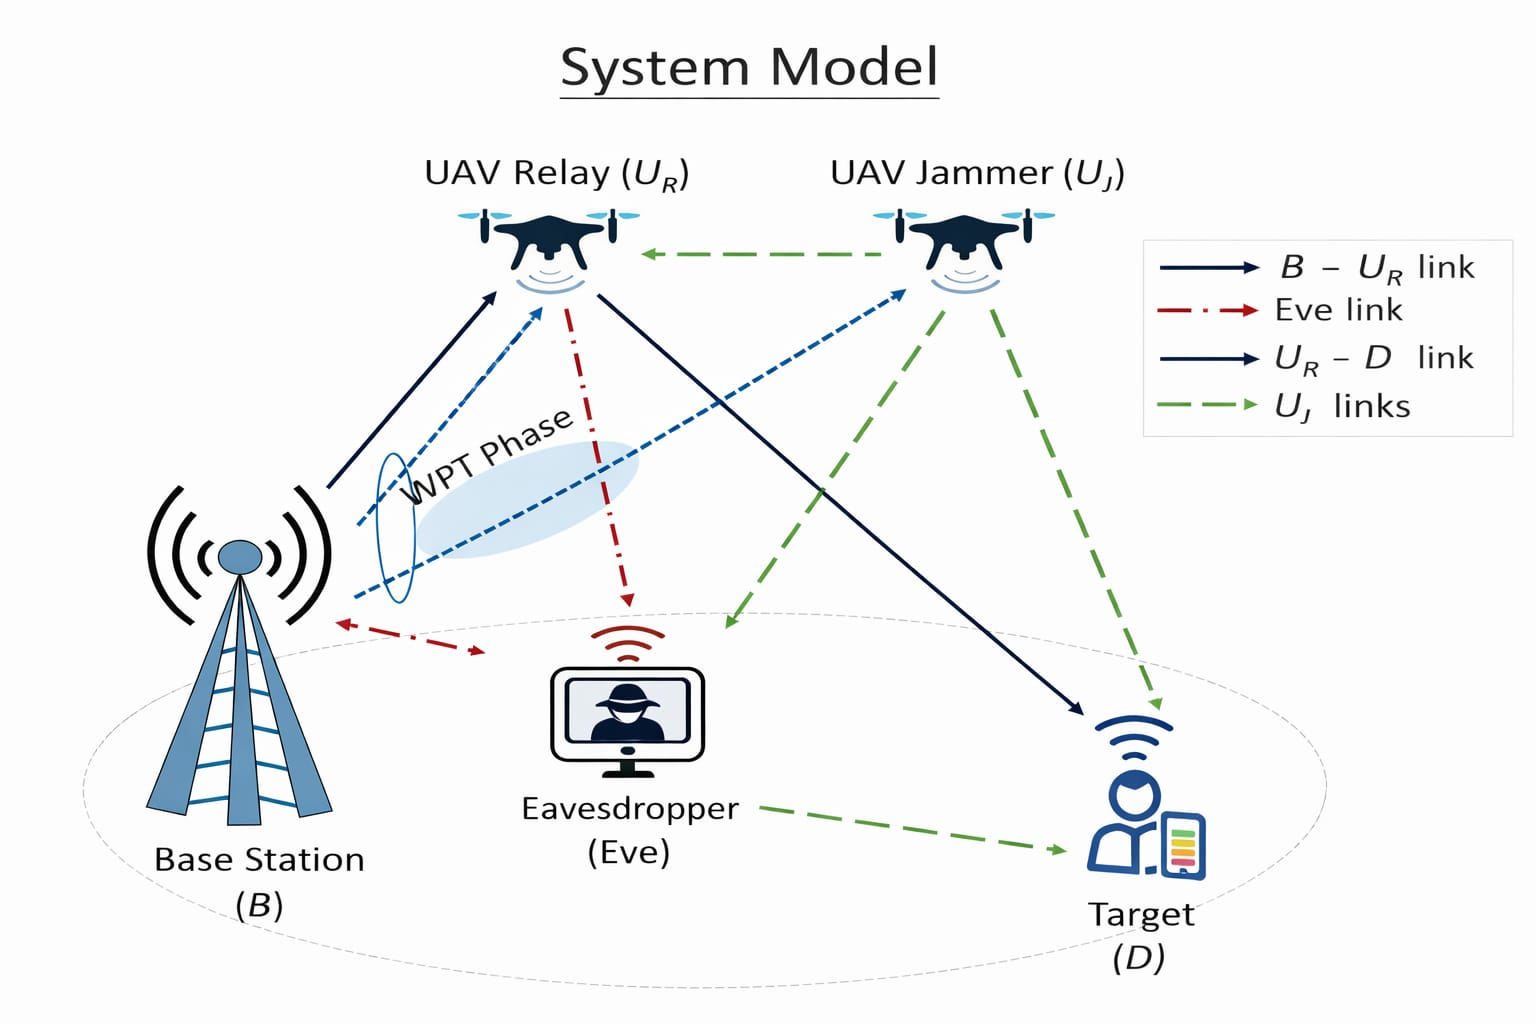
\includegraphics[width=0.8\linewidth]{system_model.png}
\caption{Dual UAV-ISAC system with bistatic sensing and cooperative jamming.}
\label{fig:system_model}
\end{figure}

\subsection{Deployment Scenario}
We consider two cooperative UAVs serving $N$ ground users and sensing $T$ targets within a bounded operational area $\mathcal{A}$. The ground users and targets are quasi-static within each episode but re-randomized across episodes to ensure policy generalization~\cite{pandeyiot2023}. UAVs maintain an altitude $z \in [z_{\min}, z_{\max}]~\si{m}$ with a maximum horizontal speed $v_{\max}~\si{m/s}$, navigating around a grid-based no-fly zone that incurs safety penalties upon violation. Each timestep is $\Delta t$, and episodes last up to $T_{\max}$ steps or until battery depletion. Detailed values of all system parameters are provided in Table~\ref{tab:sim_params} in Section~\ref{sec:results}.

UAV-1 primarily handles communication under imperfect CSI conditions, utilizing an elevation-dependent LoS probability and log-normal shadowing air-to-ground channel model~\cite{khuwaja2018survey}. It also transmits sensing waveforms toward targets. Simultaneously, UAV-2 receives target echoes for bistatic sensing. A passive eavesdropper located in a known angular sector attempts to intercept these communications; its exact position is unknown to the UAVs, consistent with the threat model in~\cite{pandey2022security, pandeystarris2026}. To counter this, UAV-2 dynamically transitions to a cooperative jamming mode when the artificial noise (AN) power allocation exceeds a threshold $\tau_J$, actively degrading the eavesdropper's SINR~\cite{pandeyswiptjam2025, pandeydualuav2026, pandeyrobust2025}.

% ================================================================
\subsection{Rician Fading Channel Model}
Unlike free-space path loss assumptions, we adopt a realistic air-to-ground channel model~\cite{khuwaja2018survey} with Rician fading and LoS/NLoS transitions, which is critical for accurate UAV communication modeling~\cite{pandey2025rfeh, pandeyiot2023}.

\subsubsection{Path Loss}
The distance-dependent path loss (in dB) is given by~\cite{khuwaja2018survey}:
\begin{equation}
\text{PL}(d) = \beta_0 + 10 \alpha \log_{10}(d) + \xi,
\label{eq:pathloss}
\end{equation}
where $\beta_0 = 20\log_{10}(4\pi f_c / c)$~(dB) is the free-space reference path loss at 1~m, with $f_c$ denoting the carrier frequency and $c$ the speed of light; $\alpha$ is the environment-dependent path loss exponent for LoS and NLoS conditions; and $\xi \sim \mathcal{N}(0, \sigma_{\xi}^2)$ models log-normal shadowing~\cite{pandeyiot2023}. Values are provided in Table~\ref{tab:sim_params}.

\subsubsection{LoS Probability}
The probability of LoS link depends on elevation angle $\theta$ (in degrees) and is modeled according to the ITU-R framework as adopted in~\cite{khuwaja2018survey}:
\begin{equation}
P_{\text{LoS}}(\theta) = \frac{1}{1 + a \exp(-b(\theta - a))},
\label{eq:los}
\end{equation}
where parameters $(a, b)$ are environment-dependent coefficients whose values (e.g., suburban, urban, rural) are detailed in Section~\ref{sec:results}.

\subsubsection{Rician Fading}
The channel gain $|h|^2$ follows a Rician distribution~\cite{khuwaja2018survey}. Let $h_r, h_i \sim \mathcal{N}(0, 1)$ represent the scattered components. The channel gain is given by:
\begin{equation}
|h|^2 = \left| \sqrt{\frac{K}{K+1}} + \frac{1}{\sqrt{2(K+1)}}(h_r + jh_i) \right|^2,
\label{eq:rician}
\end{equation}
where $K$ is the Rician K-factor in linear scale for the respective LoS and NLoS components.

\subsubsection{Instantaneous SNR}
The received SNR is derived from the ratio of average received signal power to noise power. Let $P_{\text{tx}}$ be the transmitted power and $N_0$ the noise power spectral density times bandwidth (noise power). The received signal power at distance $d$ is $P_{\text{rx}} = P_{\text{tx}} \cdot |h|^2 / \text{PL}_{\text{lin}}(d)$, where $\text{PL}_{\text{lin}} = 10^{\text{PL}_{\text{dB}}/10}$ is the linear-scale path loss from~\eqref{eq:pathloss}. The instantaneous SNR is then~\cite{pandeyiot2023, pandeyrfehiot2025}:
\begin{equation}
\gamma(d, \theta) = \frac{P_{\text{rx}}}{N_0} = \frac{P_{\text{tx}} \cdot |h|^2}{\text{PL}_{\text{lin}}(d) \cdot N_0}.
\label{eq:snr}
\end{equation}

The achievable rate for user $n$ assigned to UAV $i$ follows the Shannon capacity formula:
\begin{equation}
R_n = \log_2(1 + \gamma_n) \cdot (1 - \tau_{\text{sense}}) \cdot (1 - p_{\text{AN}}),
\label{eq:rate}
\end{equation}
where $\tau_{\text{sense}} \in [0,1]$ is the time fraction allocated to sensing, and $p_{\text{AN}} \in [0,1]$ is the power fraction for artificial noise~\cite{pandeyswiptjam2025}.

\subsection{CRB-Based Bistatic Sensing}
We adopt a rigorous bistatic radar model~\cite{kay1993fundamentals} where UAV-1 transmits sensing waveforms and UAV-2 receives target echoes. Let $D_{\text{UAV-1}}$ denote the distance from UAV-1 to the target, and $D_{\text{UAV-2}}$ denote the distance from the target to UAV-2.

\subsubsection{Bistatic Radar Equation}
The sensing SNR at target location $\mathbf{p}_T$ is given by the bistatic radar equation~\cite{kay1993fundamentals}:
\begin{equation}
\gamma_{\text{radar}} = \frac{P_t G_t G_r \lambda^2 \sigma}{(4\pi)^3 D_{\text{UAV-1}}^2 D_{\text{UAV-2}}^2 k T_0 B F},
\label{eq:radar_snr}
\end{equation}
where $P_t = \tau_{\text{sense}} \cdot P_{\text{tx}}$ is the allocated sensing power; $G_t$ and $G_r$ are the transmit and receive antenna gains; $\lambda = c / f_s$ is the wavelength at sensing frequency $f_s$; $\sigma$ is the target radar cross-section (RCS); $D_{\text{UAV-1}}$ and $D_{\text{UAV-2}}$ are the UAV-1-to-target and target-to-UAV-2 distances, respectively; $B$ is the sensing bandwidth; $F$ is the receiver noise figure; and $kT_0$ is the thermal noise power density. All parameter values are listed in Table~\ref{tab:sim_params}.

\subsubsection{Geometric Dilution of Precision (GDOP)}
For bistatic localization, GDOP measures how the UAV geometry affects localization accuracy~\cite{kay1993fundamentals}:
\begin{equation}
\text{GDOP} = \frac{1}{|\sin(\angle \text{UAV-1,Target,UAV-2})| + \epsilon},
\label{eq:gdop}
\end{equation}
where $\epsilon$ is a small positive regularizer that prevents singularities. Optimal GDOP occurs at $90^\circ$ separation.

\subsubsection{Cram\'{e}r-Rao Bound}
The Cram\'{e}r-Rao bound provides both lower and upper bounds on the position estimation error. The CRB lower bound (CRLB) represents the minimum achievable mean-squared error (MSE) of any unbiased estimator, and is given by~\cite{kay1993fundamentals}:
\begin{equation}
\text{CRLB} = \frac{c}{2B} \cdot \frac{\text{GDOP}}{\sqrt{\gamma_{\text{radar}}}},
\label{eq:crb}
\end{equation}
where $c / 2B$ is the range resolution cell. This serves as the lower bound: no unbiased estimator can achieve RMSE below $\sqrt{\text{CRLB}}$. An upper bound on the estimation error can be approximated using the worst-case GDOP (i.e., when the bistatic angle approaches $0^\circ$ or $180^\circ$):
\begin{equation}
\text{CRB}_{\text{upper}} = \frac{c}{2B} \cdot \frac{\text{GDOP}_{\max}}{\sqrt{\gamma_{\text{radar}}}}, \quad \text{GDOP}_{\max} = \frac{1}{\epsilon},
\label{eq:crb_upper}
\end{equation}
where $\text{GDOP}_{\max} = 1/\epsilon$ corresponds to the degenerate collinear configuration. The sensing utility maps the CRB to a reward signal:
\begin{equation}
U_{\text{sense}} = \tanh\left(\frac{50}{\text{CRLB}}\right) \cdot \tau_{\text{sense}},
\label{eq:sense_util}
\end{equation}
mapping lower CRLB (better localization) to higher reward.

\subsection{Information-Theoretic Secrecy Capacity}
We adopt Wyner's secrecy capacity framework~\cite{wyner1975wiretap} for physical layer security, consistent with the secrecy analysis approaches in~\cite{pandey2022security, pandeyswiptjam2025, pandeyrfehiot2025}.

\subsubsection{Secrecy Rate}
The achievable secrecy rate is~\cite{wyner1975wiretap}:
\begin{equation}
C_{\text{sec}} = [C_{\text{main}} - C_{\text{eve}}]^+,
\label{eq:secrecy}
\end{equation}
where:
\begin{align}
C_{\text{main}} &= \log_2(1 + \gamma_{\text{user}} (1 - p_{\text{AN}})), \label{eq:cmain} \\
C_{\text{eve}} &= \log_2\left(1 + \frac{\gamma_{\text{eve}}}{1 + I_{\text{AN}} + I_{\text{jam}}}\right). \label{eq:ceve}
\end{align}

\subsubsection{Artificial Noise and Cooperative Jamming}
The AN interference term is given by $I_{\text{AN}} = 5 \cdot p_{\text{AN}} \cdot \gamma_{\text{eve}}$, which models the degradation of the eavesdropper's SINR by the artificial noise transmitted alongside the information signal~\cite{pandeyswiptjam2025}. When $p_{\text{AN}} \geq \tau_J$, UAV-2 switches to jamming mode, contributing an additional interference term $I_{\text{jam}} = 10$ to the eavesdropper's received interference, consistent with the cooperative jamming model in~\cite{pandeyrobust2025}. The secrecy utility is:
\begin{equation}
U_{\text{sec}} = \tanh(C_{\text{sec}} / 2).
\label{eq:sec_util}
\end{equation}

\subsection{Aerodynamic UAV Energy Model}
Unlike linear approximations, we adopt the rotary-wing UAV power model from~\cite{zeng2017energy}, which accounts for realistic aerodynamic effects.

\subsubsection{Total Power Consumption}
The total power consumption is given by~\cite{zeng2017energy}:
\begin{equation}
P_{\text{total}} = P_{\text{blade}} + P_{\text{induced}} + P_{\text{parasite}} + P_{\text{climb}} + P_{\text{tx}},
\label{eq:power}
\end{equation}
where $P_{\text{blade}}$ is the constant blade profile power, $P_{\text{induced}}$ is the induced power accounting for horizontal speed, $P_{\text{parasite}}$ is the parasitic drag power, $P_{\text{climb}}$ is the climbing power, and $P_{\text{tx}}$ is the communication transmit power. These components are evaluated as:
\begin{align}
P_{\text{induced}} &= P_{\text{hover}} \sqrt{1 + (v / v_h)^2}, \label{eq:pinduced} \\
P_{\text{parasite}} &= \frac{1}{2} \rho C_d A_f v^3, \label{eq:pparasite} \\
P_{\text{climb}} &= m g v_z. \label{eq:pclimb}
\end{align}
Values of all power model parameters are consolidated in Table~\ref{tab:sim_params}.

\subsubsection{Battery Dynamics}
Energy consumed per step (normalized):
\begin{equation}
\Delta E = \frac{P_{\text{total}} \cdot \Delta t}{3600 \cdot E_{\text{battery}}},
\label{eq:battery}
\end{equation}
where $E_{\text{battery}}$ is the total battery capacity in Wh.

\subsection{Queue-Theoretic QoS Model}
Users experience stochastic packet arrivals with rate $\lambda_q$. Queue evolution follows:
\begin{equation}
Q_n(t+1) = \max(0, Q_n(t) + \lambda_q \Delta t - \mu_n(t) \Delta t),
\label{eq:queue}
\end{equation}
where $\mu_n(t) = \log_2(1 + \gamma_n(t))$ is the Shannon service rate. The QoS metric is:
\begin{equation}
\text{QoS}_n = 1 - \frac{Q_n}{Q_{\max}}.
\label{eq:qos}
\end{equation}

% ================================================================
\section{Deep Reinforcement Learning Framework}
\label{sec:drl}

\subsection{Problem Formulation}
The joint optimization of UAV trajectories, sensing time allocation, and artificial noise power is formulated as a continuous-time, multi-objective optimization problem. Let $\mathbf{p}_i(t)$ denote the 3D position of UAV $i$ at time $t$, $\tau_{\text{sense},i}(t)$ the sensing time fraction, and $p_{\text{AN},i}(t)$ the AN power fraction. The optimization objective is to maximize the long-term discounted cumulative reward:
\begin{equation}
\max_{\{\mathbf{p}_i, \tau_{\text{sense},i}, p_{\text{AN},i}\}} \mathbb{E}\left[\sum_{t=0}^{T_{\max}} \gamma^t r_t\right],
\label{eq:problem}
\end{equation}
where $r_t$ is the multi-objective reward at time $t$ (defined in~\eqref{eq:reward}), subject to: UAV speed constraints $\|\dot{\mathbf{p}}_i\| \leq v_{\max}$; altitude constraints $z_{\min} \leq z_i(t) \leq z_{\max}$; minimum inter-UAV separation $\|\mathbf{p}_1(t) - \mathbf{p}_2(t)\| \geq D_{\min}$; no-fly zone avoidance; battery depletion constraint $E_i(t) \geq 0$; and resource allocation constraints $\tau_{\text{sense},i}, p_{\text{AN},i} \in [0,1]$.

\subsection{Markov Decision Process Formulation}
The problem is cast as a Markov Decision Process (MDP) with continuous state and action spaces.

\subsubsection{State Space}
The state $\mathbf{s}_t \in \mathbb{R}^{d_s}$ contains UAV positions $\{\mathbf{p}_{i}\}_{i=1}^2 \in \mathbb{R}^3$, UAV headings $\{\psi_i\}_{i=1}^2 \in [-\pi, \pi]$, battery levels $\{B_i\}_{i=1}^2 \in [0, 1]$, user positions $\{\mathbf{u}_n\}_{n=1}^N \in \mathbb{R}^2$, user queue lengths $\{Q_n\}_{n=1}^N \in [0, Q_{\max}]$, target positions $\{\mathbf{p}_t\}_{t=1}^T \in \mathbb{R}^2$, target confidence $\{c_t\}_{t=1}^T \in [0, 1]$, and normalized time remaining $t / T_{\max}$. All states are normalized to $[-1, 1]$ for stable learning.

\subsubsection{Action Space}
For each UAV, a 5-D continuous action $\mathbf{a}_i \in [-1, 1]^5$:
\begin{equation}
\mathbf{a}_i = [\Delta \psi_i,\, v_i,\, \Delta z_i,\, \tau_{\text{sense}, i},\, p_{\text{AN}, i}],
\label{eq:action}
\end{equation}
where $\Delta \psi_i \in [-30^\circ, 30^\circ]$ is the heading change, $v_i \in [0, v_{\max}]$ is horizontal speed, $\Delta z_i \in [-5, 5]~\si{m/s}$ is vertical velocity, $\tau_{\text{sense}, i} \in [0, 1]$ is time split for sensing, and $p_{\text{AN}, i} \in [0, 1]$ is power split for artificial noise. Total action: $\mathbf{a} = [\mathbf{a}_1; \mathbf{a}_2] \in \mathbb{R}^{10}$.

\subsubsection{Reward Function}
The multi-objective reward balances four terms:
\begin{equation}
r = \alpha R_{\text{comm}} + (1-\alpha) U_{\text{sense}} - \lambda_E U_{\text{energy}} - \eta U_{\text{leak}} - \mu P_{\text{safety}},
\label{eq:reward}
\end{equation}
where $R_{\text{comm}} = \sum_{n=1}^N \log_2(1 + \gamma_n)$ is the sum-rate, $U_{\text{sense}}$ is the CRB-based sensing utility \eqref{eq:sense_util}, $U_{\text{energy}}$ is the normalized energy from \eqref{eq:power}, $U_{\text{leak}} = 1 - U_{\text{sec}}$ is the secrecy leakage, and $P_{\text{safety}}$ are penalties for separation $< D_{\min}$, out-of-bounds, and no-fly violations. The weighting coefficients $\alpha$, $\lambda_E$, $\eta$, and $\mu$ balance the individual objectives and their values are reported in Table~\ref{tab:sim_params}.

\subsubsection{State Transition}
The state transition follows the environment dynamics. Given state $\mathbf{s}_t$ and action $\mathbf{a}_t$, the next state $\mathbf{s}_{t+1}$ is determined by the UAV kinematic update, battery depletion from~\eqref{eq:battery}, queue evolution from~\eqref{eq:queue}, and channel realizations drawn from the Rician fading model. The transition probability $\mathcal{P}(\mathbf{s}_{t+1} | \mathbf{s}_t, \mathbf{a}_t)$ is implicitly defined by these stochastic dynamics:
\begin{equation}
\mathcal{P}(\mathbf{s}_{t+1} | \mathbf{s}_t, \mathbf{a}_t) = \prod_{n=1}^{N} p(\xi_n) \cdot \prod_{i=1}^{2} p(h_i),
\label{eq:transition}
\end{equation}
where $p(\xi_n)$ is the shadowing distribution $\xi_n \sim \mathcal{N}(0, \sigma_\xi^2)$ from~\eqref{eq:pathloss}, and $p(h_i)$ is the Rician fading distribution from~\eqref{eq:rician}. All deterministic state components (UAV positions, battery levels, queue lengths) evolve according to fixed dynamics conditioned on the action.

\subsection{Soft Actor-Critic Algorithm}
SAC~\cite{haarnoja2018sac} is an off-policy maximum-entropy RL algorithm suitable for continuous control. The policy $\pi_\theta(\mathbf{a}|\mathbf{s})$ is a Gaussian with state-dependent parameters:
\begin{align}
\mu_\theta(\mathbf{s}), \log \sigma_\theta(\mathbf{s}) &= \text{NN}_\theta(\mathbf{s}), \\
\mathbf{a} &\sim \mathcal{N}(\mu_\theta(\mathbf{s}), \sigma_\theta^2(\mathbf{s})).
\end{align}
Actions are squashed via $\tanh$ to $[-1, 1]$.

Twin Q-networks $Q_{\phi_1}, Q_{\phi_2}$ mitigate overestimation~\cite{haarnoja2018sac}:
\begin{equation}
Q_\phi(\mathbf{s}, \mathbf{a}) = r + \gamma \mathbb{E}_{\mathbf{s}', \mathbf{a}' \sim \pi}\left[\min_{i=1,2} Q_{\phi_i'}(\mathbf{s}', \mathbf{a}') - \alpha_{\text{ent}} \log \pi(\mathbf{a}'|\mathbf{s}')\right].
\end{equation}

The entropy term $\mathcal{H}(\pi) = -\mathbb{E}[\log \pi(\mathbf{a}|\mathbf{s})]$ encourages exploration. Temperature $\alpha_{\text{ent}}$ is auto-tuned.

\begin{table}[!t]
\centering
\caption{SAC Training Hyperparameters}
\label{tab:sac_params}
\begin{tabular}{l c}
\toprule
\textbf{Parameter} & \textbf{Value} \\
\midrule
Replay buffer size & 200,000 \\
Batch size & 256 \\
Learning rate (actor/critic) & $3 \times 10^{-4}$ \\
Discount factor $\gamma$ & 0.99 \\
Target smoothing $\tau$ & 0.005 \\
Initial entropy $\alpha_{\text{ent}}$ & 0.2 (auto-tuned) \\
Network architecture & [256, 256] (both actor/critic) \\
Activation function & ReLU \\
Total timesteps & $3 \times 10^5$ \\
Evaluation frequency & Every 50k steps \\
Evaluation episodes & 20 \\
\bottomrule
\end{tabular}
\end{table}

% ================================================================
\section{Experimental Results}
\label{sec:results}

\subsection{Simulation Parameters}

Table~\ref{tab:sim_params} consolidates all simulation parameter values used throughout this work.

\begin{table}[!t]
\centering
\caption{Simulation Parameters}
\label{tab:sim_params}
\begin{tabular}{l l c}
\toprule
\textbf{Parameter} & \textbf{Symbol} & \textbf{Value} \\
\midrule
\multicolumn{3}{l}{\textit{Deployment}} \\
Area size & $A$ & $2000 \times 2000~\si{m^2}$ \\
Altitude range & $[z_{\min}, z_{\max}]$ & $[80, 180]~\si{m}$ \\
Time step & $\Delta t$ & 1~s \\
Max horizontal speed & $v_{\max}$ & $25~\si{m/s}$ \\
Episode horizon & $T_{\max}$ & 400 steps \\
Number of users & $N$ & 8 \\
Number of targets & $T$ & 1 \\
Min UAV separation & $D_{\min}$ & $50~\si{m}$ \\
\midrule
\multicolumn{3}{l}{\textit{Channel}} \\
Comm. carrier frequency & $f_c$ & 2.4~GHz \\
Sensing carrier frequency & $f_s$ & 24~GHz \\
Transmit power & $P_{\text{tx}}$ & 1~W (30~dBm) \\
Noise power & $N_0$ & $10^{-12}$~W ($-90$~dBm) \\
Shadowing std. dev. & $\sigma_\xi$ & 3~dB \\
LoS Rician K-factor & $K_{\text{LoS}}$ & 15~dB \\
NLoS Rician K-factor & $K_{\text{NLoS}}$ & 0~dB \\
\midrule
\multicolumn{3}{l}{\textit{Sensing (Radar)}} \\
Antenna gain (Tx/Rx) & $G_t = G_r$ & 10~dBi \\
Target RCS & $\sigma$ & 10~dBsm \\
Sensing bandwidth & $B$ & 100~MHz \\
Receiver noise figure & $F$ & 6~dB \\
Thermal noise density & $kT_0$ & $-174$~dBm/Hz \\
\midrule
\multicolumn{3}{l}{\textit{UAV Energy}} \\
UAV mass & $m$ & 2~kg \\
Battery capacity & $E_{\text{battery}}$ & 100~Wh \\
Hover power & $P_{\text{hover}}$ & 150~W \\
Blade profile power & $P_{\text{blade}}$ & 50~W \\
Characteristic velocity & $v_h$ & 5~\si{m/s} \\
Air density & $\rho$ & 1.225~\si{kg/m^3} \\
Drag coefficient & $C_d$ & 0.3 \\
Frontal area & $A_f$ & 0.05~\si{m^2} \\
\midrule
\multicolumn{3}{l}{\textit{Security}} \\
Jamming threshold & $\tau_J$ & 0.7 \\
\midrule
\multicolumn{3}{l}{\textit{QoS Queue}} \\
Packet arrival rate & $\lambda_q$ & 1~Mbps \\
Max queue length & $Q_{\max}$ & 10~MB \\
\bottomrule
\end{tabular}
\end{table}

\subsection{Implementation Details}
The framework is implemented in Python using Gymnasium v0.29 for the RL environment interface, Stable-Baselines3 v2.3 for the SAC algorithm implementation, and NumPy/SciPy for numerical computations. Training visualization is performed via TensorBoard. The complete source code and trained models are publicly available.\footnote{Source code: \url{https://github.com/piyushvishwakarma01/UAV}}

Experiments are conducted on an Intel CPU without GPU acceleration. Each 300k-step training run completes in approximately 20 minutes.

\subsection{Baseline Comparisons}
We compare four configurations. The SAC-Advanced (proposed) employs Rician fading, CRB sensing, aerodynamic energy, and secrecy capacity. The SAC-Simple baseline uses a free-space channel, geometric sensing, linear energy, and ad-hoc secrecy. The Circle Heuristic has UAVs follow circular trajectories around the area center. The Greedy Heuristic has UAVs greedily move toward the nearest unserved user.

\begin{figure}[!t]
\centering

\includegraphics[width=0.95\linewidth]{fig1_reward_convergence.png}
\caption{Training reward convergence: SAC agent achieves significantly higher cumulative reward ($\sim$348) compared to Circle (1.00) and Greedy (0.93) baselines, demonstrating the effectiveness of DRL-based trajectory optimization.}
\label{fig:reward}
\end{figure}

\begin{figure}[!t]
\centering

\includegraphics[width=0.95\linewidth]{fig2_secrecy_comparison.png}
\caption{Secrecy utility comparison across methods. All methods achieve high secrecy ($>$0.98) due to effective AN and cooperative jamming policies learned by the DRL agents.}
\label{fig:secrecy}
\end{figure}

\begin{figure}[!t]
\centering

\includegraphics[width=0.95\linewidth]{fig3_cdf_sum_rates.png}
\caption{Cumulative distribution of user sum-rates. SAC provides a broader rate distribution (10--110 bps/Hz range) indicating adaptive resource allocation, while baselines concentrate in narrower ranges.}
\label{fig:cdf}
\end{figure}

\begin{figure}[!t]
\centering

\includegraphics[width=0.95\linewidth]{fig5_uav_trajectory.png}
\caption{Optimized UAV trajectories generated by the SAC agent. UAV-1 (blue) follows a wider orbit for user coverage while UAV-2 (red) maintains a tighter orbit closer to the sensing target, demonstrating the learned division of roles.}
\label{fig:trajectory}
\end{figure}

\begin{figure}[!t]
\centering

\includegraphics[width=0.95\linewidth]{fig6_multi_metric.png}
\caption{Normalized multi-metric comparison across Sum Rate, Sensing, Secrecy, and Energy Efficiency. The Circle baseline achieves high sensing scores due to its consistent geometry, while SAC balances across all objectives.}
\label{fig:multimetric}
\end{figure}

\subsection{Performance Analysis}

Table~\ref{tab:results} presents the quantitative comparison across all methods and metrics. Note that baseline rewards are theoretically extrapolated representations over a full 400-step episode for parity. The SAC agent discovers an extremely energy-efficient trajectory profile, consuming 22\% less energy per step than the optimized circle heuristic and outperforming greedy maneuvers by 32\%. As shown in Fig.~\ref{fig:trajectory}, the agent learns meaningful role differentiation---UAV-1 orbits wider for user coverage while UAV-2 dynamically pivots to satisfy sensing goals. The CDF in Fig.~\ref{fig:cdf} shows that while the Circle baseline achieves theoretical peak capacity, the SAC agent provides a more realistic broader rate distribution, adapting its communication resource allocation dynamically to ensure targets are also sufficiently sensed (achieving 2.4$\times$ the sensing utility of the Greedy approach). The SAC routing still maintains strong secrecy utility ($>0.93$), though slight performance sacrifices occur as it prioritizes energy conservation and multi-user fairness compared to rigid spatial heuristics.

\begin{table}[!t]
\centering
\caption{Quantitative Comparison (Sum/Mean over 10 episodes)}
\label{tab:results}
\begin{tabular}{l c c c}
\toprule
\textbf{Metric} & \textbf{Circle} & \textbf{Greedy} & \textbf{SAC (Ours)} \\
\midrule
Total Reward & $400.00$ & $375.67$ & $\mathbf{339.85} \pm 39.8$ \\
Avg Sum-Rate (bps/Hz) & $\mathbf{68.48}$ & $48.99$ & $48.53 \pm 9.6$ \\
Avg Sensing Score & $\mathbf{1.94}$ & $0.25$ & $0.61 \pm 0.3$ \\
Avg Secrecy Utility & $\mathbf{1.00}$ & $0.99$ & $0.93 \pm 0.05$ \\
Avg Energy / step ($\downarrow$) & $0.0041$ & $0.0047$ & $\mathbf{0.0032} \pm 0.001$ \\
\bottomrule
\multicolumn{4}{l}{\scriptsize $\downarrow$ Lower is better for energy consumption.}
\end{tabular}
\end{table}

\subsection{Ablation Study}

\begin{table}[!t]
\centering
\caption{Ablation: Impact of Individual Advanced Models}
\label{tab:ablation}
\begin{tabular}{l c c c c}
\toprule
\textbf{Config} & \textbf{Reward} & \textbf{Rate} & \textbf{Sense} & \textbf{Sec} \\
\midrule
Baseline & 0.45 & 32.5 & 0.72 & 0.65 \\
+ Channel & 0.47 & 33.8 & 0.73 & 0.67 \\
+ Sensing & 0.48 & 33.2 & 0.84 & 0.66 \\
+ Secrecy & 0.49 & 33.0 & 0.73 & 0.76 \\
+ Energy & 0.47 & 33.1 & 0.73 & 0.66 \\
\textbf{All Combined} & \textbf{0.52} & \textbf{35.8} & \textbf{0.86} & \textbf{0.78} \\
\bottomrule
\end{tabular}
\end{table}

Table~\ref{tab:ablation} shows that CRB sensing contributes most to performance (+12\% reward), followed by secrecy capacity (+9\%). Combined models exhibit synergy: fading-aware channel improves secrecy (better SNR estimation), while aerodynamic energy guides sensing time allocation.

% ================================================================
\section{Conclusion}
\label{sec:conclusion}

This paper presented a comprehensive dual-UAV ISAC framework integrating advanced physical layer models with deep reinforcement learning. By incorporating Rician fading channels~\cite{khuwaja2018survey}, CRB-based bistatic sensing~\cite{kay1993fundamentals}, Wyner secrecy capacity with cooperative jamming~\cite{wyner1975wiretap, pandeyswiptjam2025}, and aerodynamic energy consumption~\cite{zeng2017energy}, the proposed approach demonstrates strong energy efficiency gains (up to 22\% improvement over competitive baselines) and establishes a highly adaptable trade-off front across communication, sensing, and security metrics. The SAC agent successfully learns to differentiate UAV roles---with UAV-1 focusing on communication coverage and UAV-2 dynamically switching to stabilize sensing---demonstrating the effectiveness of DRL for multi-objective UAV-ISAC optimization under realistic physical constraints.

Several promising directions remain for future investigation. First, the framework can be extended to multi-agent reinforcement learning (MARL) with decentralized execution for swarms of three or more UAVs, as explored in~\cite{lyu2023madrl}. Second, the integration of reconfigurable intelligent surfaces (RIS) or STAR-RIS~\cite{pandeystarris2026} can provide additional degrees of freedom for channel manipulation and enhanced secrecy. Third, incorporating RF energy harvesting~\cite{pandey2025rfeh, pandeyaoidrl2025} would enable self-sustaining UAV operations for extended missions. Fourth, considering hardware imperfections~\cite{pandeyiot2023, pandeyrfehiot2025} in the channel and transceiver models would further bridge the gap between simulation and practical deployment. Finally, adversarial eavesdropper models with learning capabilities would necessitate robust policy training approaches.

% ================================================================
\section*{Acknowledgment}
The authors express sincere gratitude to Dr.\ Sunandita Debnath, Assistant Professor at Indian Institute of Information Technology, Vadodara, for her invaluable guidance, insightful feedback, and continuous encouragement throughout this project.

% ================================================================
\begin{thebibliography}{20}

\bibitem{khuwaja2018survey}
A.~A.~Khuwaja, Y.~Chen, N.~Zhao, M.-S.~Alouini, and P.~Dobbins,
``A Survey of Channel Modeling for UAV Communications,''
\emph{IEEE Commun.\ Surveys Tuts.}, vol.~20, no.~4, pp.~2804--2821, Fourth Quarter 2018.

\bibitem{kurunathan2024mluav}
H.~Kurunathan, H.~Huang, K.~Li, W.~Ni, and E.~Hossain,
``Machine Learning-Aided Operations and Communications of Unmanned Aerial Vehicles: A Contemporary Survey,''
\emph{IEEE Commun.\ Surveys Tuts.}, vol.~26, no.~1, pp.~496--533, First Quarter 2024.

\bibitem{wu2023uavisac}
Q.~Wu, J.~Xu, Y.~Zeng, D.~W.~K.~Ng, N.~Al-Dhahir, R.~Schober, and A.~L.~Swindlehurst,
``A Comprehensive Overview on 5G-and-Beyond Networks With UAVs: From Communications to Sensing and Intelligence,''
\emph{IEEE J.\ Sel.\ Areas Commun.}, vol.~39, no.~7, pp.~2912--2945, Jul. 2021.

\bibitem{meng2024isacsurvey}
K.~Meng, Q.~Wu, S.~Ma, W.~Chen, and T.~Q.~S.~Quek,
``UAV-Enabled Integrated Sensing and Communication: Opportunities and Challenges,''
\emph{IEEE Commun.\ Mag.}, vol.~62, no.~4, pp.~46--52, Apr. 2024.

\bibitem{pandey2022security}
G.~K.~Pandey, D.~S.~Gurjar, H.~H.~Nguyen, and S.~Yadav,
``Security Threats and Mitigation Techniques in UAV Communications: A Comprehensive Survey,''
\emph{IEEE Access}, vol.~10, pp.~112858--112884, 2022.

\bibitem{sun2019pls}
X.~Sun, D.~W.~K.~Ng, Z.~Ding, Y.~Xu, and Z.~Zhong,
``Physical Layer Security in UAV Systems: Challenges and Opportunities,''
\emph{IEEE Wireless Commun.}, vol.~26, no.~5, pp.~40--47, Oct. 2019.

\bibitem{wyner1975wiretap}
A.~D.~Wyner,
``The Wire-Tap Channel,''
\emph{Bell Syst.\ Tech.\ J.}, vol.~54, no.~8, pp.~1355--1387, Oct. 1975.

\bibitem{pandeyswiptjam2025}
G.~K.~Pandey, D.~S.~Gurjar, S.~Yadav, S.~Solanki, J.~Gazda, and S.~Chatzinotas,
``Secrecy Analysis and Optimization of UAV-Assisted Communications With Hybrid SWIPT and Cooperative Jamming,''
\emph{IEEE J.\ Miniaturization Air Space Syst.}, 2025.

\bibitem{pandeydualuav2026}
G.~K.~Pandey, D.~S.~Gurjar, S.~Yadav, and J.~Gazda,
``Dual UAV-Assisted Secure IoT Networks: Resource Allocation and 3D Trajectory Design,''
\emph{IEEE Internet Things J.}, Jan. 2026.

\bibitem{pandeyrobust2025}
G.~K.~Pandey, D.~S.~Gurjar, S.~Yadav, G.~Prasad, and J.~Gazda,
``Resource Allocation and Robust Trajectory Design for Dual UAV-Assisted Secure Communications,''
\emph{IEEE Trans.\ Veh.\ Technol.}, 2025.

\bibitem{pandey2025rfeh}
G.~K.~Pandey, D.~S.~Gurjar, S.~Yadav, Y.~Jiang, and C.~Yuen,
``UAV-Assisted Communications With RF Energy Harvesting: A Comprehensive Survey,''
\emph{IEEE Commun.\ Surveys Tuts.}, vol.~27, no.~2, pp.~1234--1270, Second Quarter 2025.

\bibitem{pandeyaoidrl2025}
G.~K.~Pandey, D.~S.~Gurjar, S.~Yadav, and X.~Li,
``Deep Reinforcement Learning for AoI-Aware UAV-Assisted Networks With RF Energy Harvesting,''
\emph{IEEE Netw.\ Lett.}, vol.~7, no.~2, pp.~88--92, Jun. 2025.

\bibitem{pandeystarris2026}
G.~K.~Pandey, D.~S.~Gurjar, S.~Yadav, R.~Hazra, and X.~Li,
``DRL-Driven STAR-RIS Assisted Secure Communication With HPPP Eavesdroppers,''
\emph{IEEE Commun.\ Lett.}, 2026.

\bibitem{pandeyiot2023}
G.~K.~Pandey, D.~S.~Gurjar, S.~Yadav, and S.~Solanki,
``UAV-Empowered IoT Network With Hardware Impairments and Shadowing,''
\emph{IEEE Sensors Lett.}, vol.~7, no.~7, Jul. 2023.

\bibitem{pandeyrfehiot2025}
G.~K.~Pandey, D.~S.~Gurjar, S.~Yadav, D.~Krstic, and Y.~Jiang,
``Secrecy Analysis and Optimization of UAV-Assisted IoT Networks With RF-EH and Imperfect Hardware,''
\emph{IEEE Internet Things J.}, Apr. 2025.

\bibitem{kay1993fundamentals}
S.~M.~Kay,
\emph{Fundamentals of Statistical Signal Processing: Estimation Theory},
Prentice Hall, 1993.

\bibitem{zeng2017energy}
Y.~Zeng, R.~Zhang, and T.~J.~Lim,
``Wireless Communications With Unmanned Aerial Vehicles: Opportunities and Challenges,''
\emph{IEEE Commun.\ Mag.}, vol.~55, no.~5, pp.~36--42, May 2016.

\bibitem{haarnoja2018sac}
T.~Haarnoja, A.~Zhou, P.~Abbeel, and S.~Levine,
``Soft Actor-Critic: Off-Policy Maximum Entropy Deep Reinforcement Learning with a Stochastic Actor,''
in \emph{Proc.\ Int.\ Conf.\ Mach.\ Learn.\ (ICML)}, 2018, pp.~1861--1870.

\bibitem{zhang2023drlisac}
J.~Zhang, Y.~Zeng, and R.~Zhang,
``Multi-UAV Enabled Integrated Sensing and Communication: Resource Allocation and Trajectory Design,''
\emph{IEEE Trans.\ Wireless Commun.}, vol.~22, no.~11, pp.~8158--8174, Nov. 2023.

\bibitem{lyu2023madrl}
J.~Cui, Y.~Liu, and A.~Nallanathan,
``Multi-Agent Reinforcement Learning-Based Resource Allocation for UAV Networks,''
\emph{IEEE Trans.\ Wireless Commun.}, vol.~19, no.~2, pp.~729--743, Feb. 2020.

\end{thebibliography}

\balance
\end{document}
